\documentclass{standalone}
\usepackage{tikz} %Graphics
\usetikzlibrary{shapes.geometric, arrows}
\tikzstyle{title} = [text centered]
\tikzstyle{block} = [rectangle, rounded corners, minimum width=3cm, minimum height=1.5cm,text centered, draw=black, fill=blue!30]
\tikzstyle{blue_block} = [rectangle, rounded corners, minimum width=3cm, minimum height=1.5cm,text centered, draw=black, fill=blue!30]
\tikzstyle{green_block} = [rectangle, rounded corners, minimum width=3cm, minimum height=1.5cm,text centered, draw=black, fill=green!30]
\tikzstyle{orange_block} = [rectangle, rounded corners, minimum width=3cm, minimum height=1.5cm,text centered, draw=black, fill=orange!30]
\tikzstyle{red_block} = [rectangle, rounded corners, minimum width=3cm, minimum height=1.5cm,text centered, draw=black, fill=red!30]
\tikzstyle{arrow} = [thick,->,>=stealth]

%\usetikzlibrary{...}
\begin{document}
	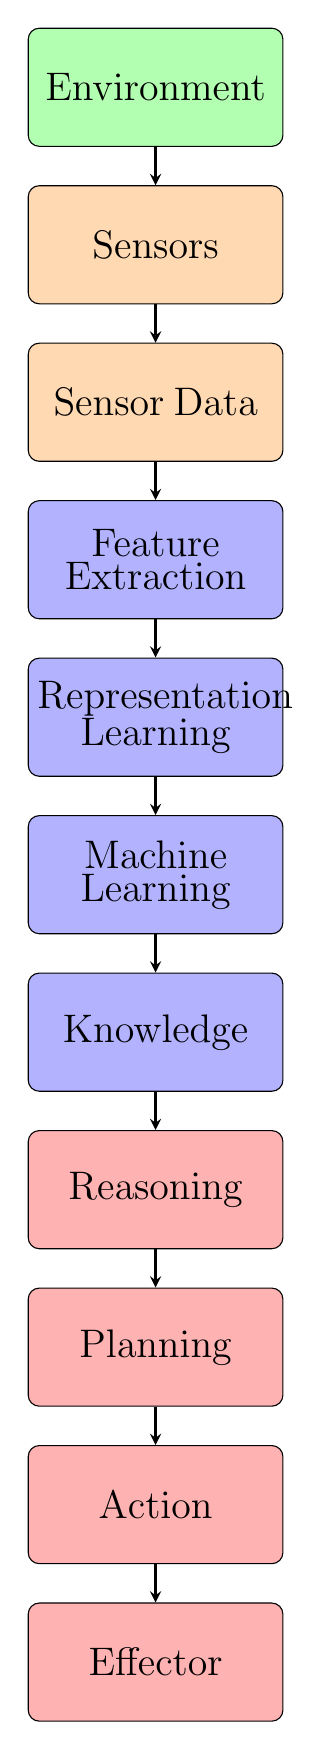
\begin{tikzpicture}[node distance=2cm]
		%\node (decomp) [title] { Initial Classifier };
		\node (l0) [green_block, xshift=11mm, text width=3cm] {\Large Environment};			
		\node (l1) [orange_block, below of = l0, text width=3cm] {\Large Sensors};
		\node (l2) [orange_block, below of=l1, text width=3cm] {\Large Sensor Data};
		\node (l3) [blue_block, below of=l2, text width=3cm] {\Large Feature Extraction};
		\node (l4) [blue_block, below of=l3, text width=3cm] {\Large Representation Learning};
		\node (l5) [blue_block, below of=l4, text width=3cm] {\Large Machine Learning};			
		\node (l6) [blue_block, below of = l5, text width=3cm] {\Large Knowledge};
		\node (l7) [red_block, below of=l6, text width=3cm] {\Large Reasoning};
		\node (l8) [red_block, below of=l7, text width=3cm] {\Large Planning};
		\node (l9) [red_block, below of=l8, text width=3cm] {\Large Action};
		\node (l10) [red_block, below of=l9, text width=3cm] {\Large Effector};
				
		\draw [arrow] (l0) -- (l1);		
		\draw [arrow] (l1) -- (l2);
		\draw [arrow] (l2) -- (l3);
		\draw [arrow] (l3) -- (l4);		
		\draw [arrow] (l4) -- (l5);		
		\draw [arrow] (l5) -- (l6);
		\draw [arrow] (l6) -- (l7);
		\draw [arrow] (l7) -- (l8);		
		\draw [arrow] (l8) -- (l9);		
		\draw [arrow] (l9) -- (l10);

\end{tikzpicture}
\end{document}
